% !TEX encoding = UTF-8
% !TEX TS-program = pdflatex
% !TEX root = ../tesi.tex

%**************************************************************
\chapter{Progettazione e codifica}
\label{cap:progettazione-codifica}
%**************************************************************

\intro{Questo capitolo presenta lo studio della parte di interesse del framework aziendale e l'attività di progettazione svolta per il progetto, approfondita con diagrammi UML. La progettazione viene scissa in due parti: progettazione dell'estensione del framework e progettazione dell'applicazione, per mantenere separate le due parti di software prodotte durante lo svolgimento dello stage. La progettazione è avvenuta seguendo un approccio top-down: dapprima sono state individuate le componenti ad alto livello e la loro interazione, fino all’individuazione dei singoli moduli e delle classi.}\\

%**************************************************************
\section{Premessa: architettura e funzionamento \\ del framework}
\begin{figure}[!h]
    \begin{widepage}
        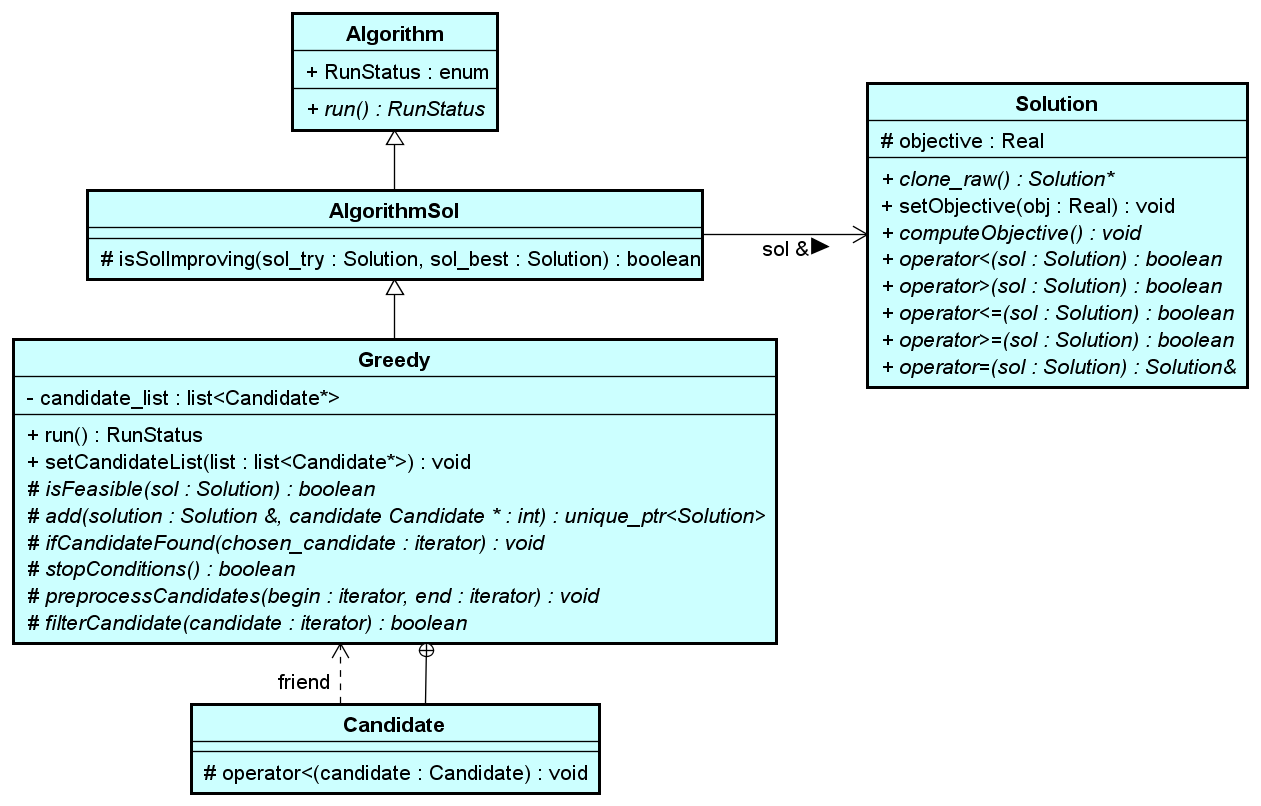
\includegraphics[width=14.9cm,keepaspectratio]{../immagini/progettazione/framework.png}
        \caption{Architettura di dettaglio di parte del framework aziendale}
    \end{widepage}
\end{figure}
Il framework aziendale, come già accennato, offre una base per l'implementazione di algoritmi di ottimizzazione e consiste di librerie per l'utilizzo di grafi, di algoritmi euristici di tipo greedy e di meta-euristiche, ad esempio Tabu Search. 
Per l'estensione del framework con la risoluzione dei problemi di scheduling, durante lo stage ho dovuto utilizzare la parte di libreria atta all'implementazione di algoritmi greedy; di seguito ne viene riportata la sua struttura e ne sono messi in evidenza i metodi di interesse.
\paragraph{Algorithm} la classe \texttt{Algorithm} è un'interfaccia per l'implementazione di qualsiasi algoritmo. Ha un unico metodo virtuale puro, \texttt{run()}, che deve essere implementato nelle sue classi derivate con il corpo dell'algoritmo di risoluzione; esso deve ritornare un \texttt{RunStatus}: SUCCESS\textunderscore RUN, FAIL\textunderscore RUN, UNFEASIBLE.
\paragraph{AlgorithmSol} è derivata da \texttt{Algorithm} ma ancora astratta in quanto non dà un'implementazione del metodo \texttt{run()}. Essa rapresenta un'ulteriore strato prima di poter implementare gli algoritmi, in quanto contiene un riferimento alla classe \texttt{Solution}. Il suo unico metodo \texttt{isSolImproving()} serve a confrontare gli objective di due \texttt{Solution} per stabilire quale delle due sia la migliore.
\paragraph{Candidate} è interna a \texttt{Greedy} rappresenta un candidato da valutare all'interno del metodo \texttt{run()}. Va estesa con classi derivate che aggiungano le strutture dati. Una lista di tutti i candidati è campo dati di \texttt{Greedy}.
\paragraph{Greedy} è derivata di AlgorithmSol e rappresenta un template di implementazione per gli algoritmi greedy. Implementa il metodo \texttt{run()} con uno ``scheletro'' generale valido per tutti gli algoritmi di tipo greedy, applicando il \emph{\gls{design}}\glsfirstoccur\ ``Template Method''. Tutti gli altri metodi virtuali rappresentano gli hook per il metodo template e devono essere implementati nelle classi derivate a seconda di che algoritmo greedy si vuole implementare.
\paragraph{Solution} è una classe astratta che rappresenta la soluzione trovata all'interno del metodo \texttt{run()}. Ha come unico campo dati \texttt{objective}, che è il risultato della funzione obiettivo implementata dentro il metodo virtuale puro \texttt{computeObjective()}. Nelle classi derivate bisogna implementare tale metodo, gli operatori di confronto, e aggiungere una struttura dati che permetta di mantenere memoria della soluzione.

\subsection{Il metodo run()}
Essendo il punto cardine dell'estensione del framework, è opportuno spiegare il funzionamento del metodo template \texttt{run()} implementato all'interno di \texttt{Greedy}. A tale scopo se ne riporta uno pseudocodice estremamente semplificato, con i metodi virtuali puri da implementare nelle classi derivate evidenziati in rosso:
\newpage
\begin{lstlisting}
while(!stopConditions()){
    preprocessCandidates(list_begin, list_end);
    chosen_candidate =list_end;
    list<Candidate*>::iterator candidate;
    for (candidate = list_begin; candidate != list_end; candidate++){
        if (filterCandidate(candidate))
            continue;
        solution_try = add(sol, candidate);
        solution_try.computeObjective();
        if (isFeasible(solution_try) && (solution_try < solution_best)){
            solution_best = move(solution_try);
            chosen_candidate = candidate;
        }  
    }
    setSol(solution_best);
    if (chosen_candidate != list_end)
        ifCandidateFound(chosen_candidate);
    else
        return UNFEASIBLE;
}
return SUCCESS_RUN;
\end{lstlisting}
\noindent
\\
Il suo funzionamento è il seguente:
\begin{enumerate}
    \item Il metodo \texttt{stopConditions()} torna \texttt{true} quando lo scheduling è stato riempito. In tal caso, il metodo run torna \texttt{SUCCESS\textunderscore RUN}. Se il metodo \texttt{StopConditions()} torna \texttt{false}, lo scheduling non è completo e quindi la \texttt{run()} continua a ciclare.
    \item Il metodo \texttt{preprocessCandidates()} permette di modificare per side effect due iteratori \texttt{list\textunderscore begin} e \texttt{list\textunderscore end} che determinano quale set dalla lista di candidati \texttt{candidate\textunderscore list} verranno valutati all'interno del ciclo.
    \item Per ogni candidato all'interno del set selezionato:
    \begin{enumerate}
        \item Il metodo \texttt{filterCandidate()} permette di saltare la valutazione del candidato. Se ritorna \texttt{true}, si passa alla valutazione del candidato successivo (punto 3).
        \item Altrimenti, il metodo \texttt{add()} aggiunge a \texttt{solution\textunderscore try} il candidato e ne valuta l'obiettivo.
        \item Il metodo \texttt{isFeasible()} valuta se \texttt{solution\textunderscore try} è ammissibile e se è migliorante rispetto a  \texttt{solution\textunderscore best}. In caso positivo, \texttt{solution\textunderscore try} diventa \texttt{solution\textunderscore best}.
    \end{enumerate}
\item Una volta valutati tutti i candidati, viene impostata \texttt{solution\textunderscore best} come soluzione contenuta in \texttt{AlgorithmSol}.
\item Se è stato scelto un candidato, il metodo \texttt{ifCandidateFound()} permette di eseguire delle operazioni sul candidato successive alla sua assegnazione. Altrimenti, se nessun candidato è stato scelto, la soluzione non è ammissibile e il metodo run torna \texttt{UNFEASIBLE}. 
\item Torno al punto 1.
\end{enumerate}
\newpage
%**************************************************************
\section{Progettazione dell'estensione del framework}
\begin{figure}[!h]
    \begin{widepage}
        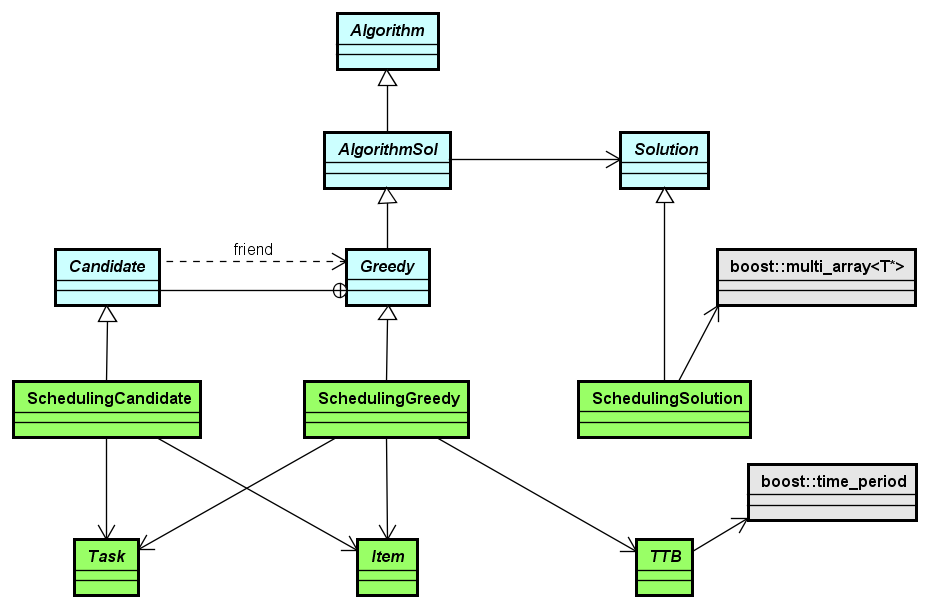
\includegraphics[width=14.9cm,keepaspectratio]{../immagini/progettazione/estensione.png}
        \caption{Architettura generale dell'estensione al framework}
    \end{widepage}
\end{figure}
\FloatBarrier
\noindent
\paragraph{Task} classe che modella un generico \task\ di un problema di scheduling e contiene le strutture dati per salvarne le informazioni relative, ad esempio l'essere aperto/chiuso, o la popolarità.
\paragraph{TTB} classe che modella un generico \ttb\ di un problema di scheduling e contiene le strutture dati per salvarne le informazioni relative, ad esempio gli orari di inizio e fine, o la popolarità.
\paragraph{Item} classe astratta che modella un generico \items\ di un problema di scheduling e contiene le strutture dati per salvarne le informazioni relative, ad esempio gli orari di lavoro, la disponibilità a svolgere straordinari, o la popolarità/fairness che acquisisce man mano che che gli vengono assegnati dei \task. La classe viene approfondita nel paragrafo 6.1 di questo capitolo, relativo alla progettazione di dettaglio.
\paragraph{SchedulingSolution} classe che eredita da \texttt{Solution} e definisce, utilizzando la libreria Boost, un \texttt{multi\textunderscore array<Item*,2>} per salvare lo scheduling prodotto dal metodo \texttt{run()}. Implementa inoltre il metodo \texttt{computeObjective()} calcolando l'obiettivo secondo gli starordinari svolti, la popolarità e la fairness accumulate da tutti gli oggetti di tipo \texttt{Item}.
\paragraph{SchedulingGreedy} classe che eredita da \texttt{Greedy} e ne implementa quindi tutti i metodi virtuali puri. La classe viene approfondita nel paragrafo 6.2 di questo capitolo, relativo alla progettazione di dettaglio.
\paragraph{SchedulingCandidate} classe che eredita da \texttt{Candidate} e modella i candidati da valutare all'interno del metodo \texttt{run()}. Ogni \texttt{SchedulingCandidate} è composto da una coppia \texttt{Item*}, \texttt{Task*} e indica che l'oggetto di tipo \texttt{Task} può essere assegnato all'oggetto di tipo \texttt{Item}.
%**************************************************************
\section{Progettazione dell'applicazione}
\begin{figure}[!h]
    \begin{widepage}
        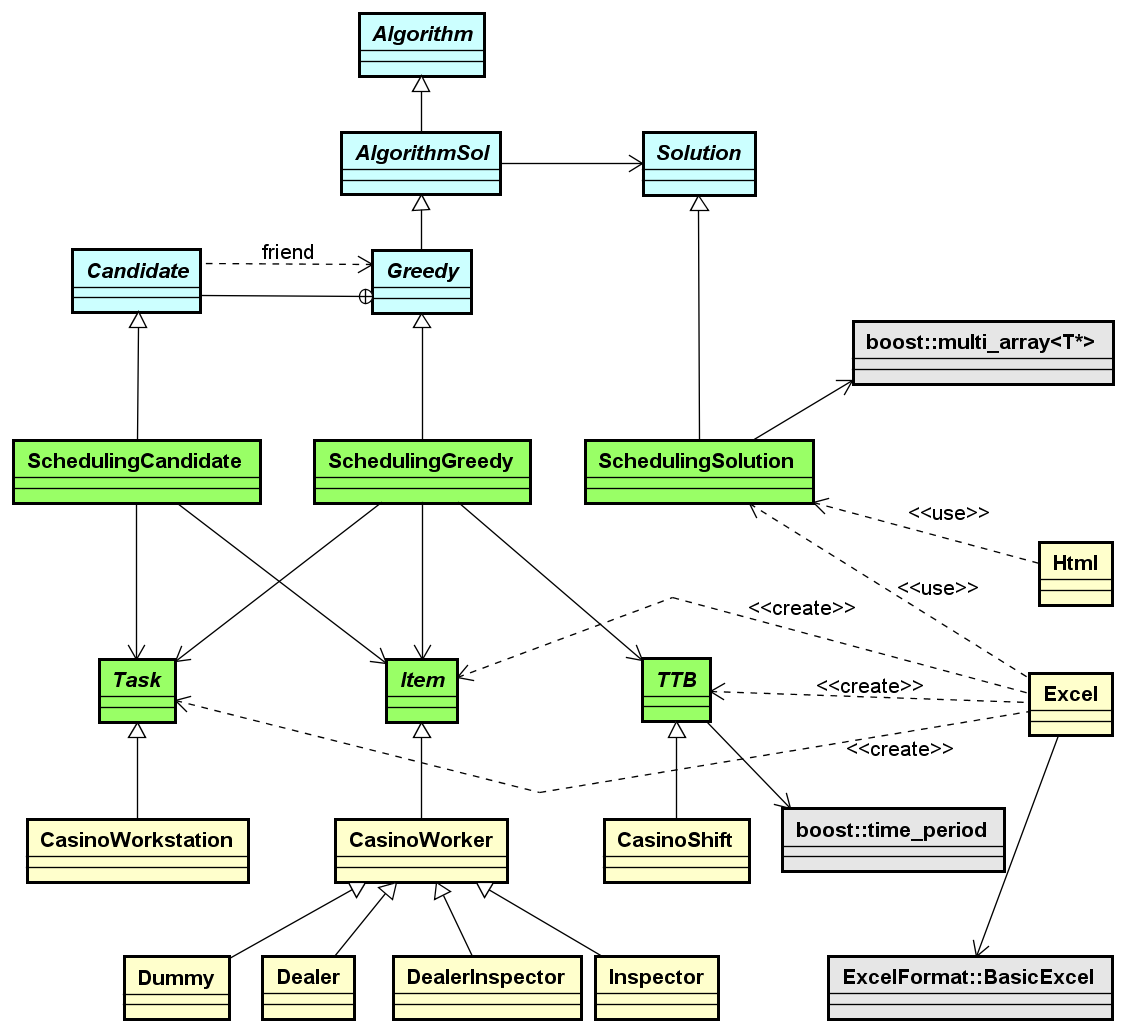
\includegraphics[width=14.9cm,keepaspectratio]{../immagini/progettazione/applicazione.png}
        \caption{Architettura generale dell'applicazione al problema del casinò}
    \end{widepage}
\end{figure}
\FloatBarrier
\noindent
\paragraph{CasinoWorkstation}
\paragraph{CasinoWorker}
\paragraph{Dealer}
\paragraph{Inspector}
\paragraph{DealerInspector}
\paragraph{Inspector}
\paragraph{CasinoShift}
\paragraph{Excel}
\paragraph{Html}
%**************************************************************
\section{Librerie}
\paragraph{Excel}
\paragraph{Boost}
%**************************************************************
\section{Design pattern}
\paragraph{Template Method}
\begin{figure}[!h]
    \centering
        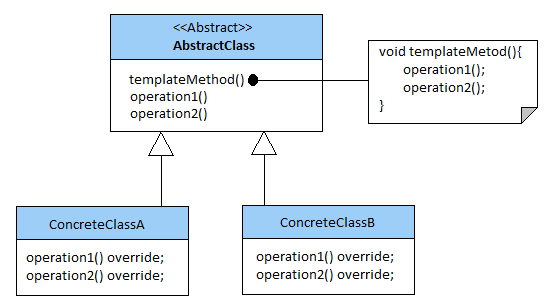
\includegraphics[width=10cm,keepaspectratio]{../immagini/templatemethod.jpg}
        \caption{Template Method}
\end{figure}
%**************************************************************
\section{Progettazione di dettaglio}
In questa sezione illustrerò le classi principali del progetto, tralasciando
quelle meno importanti.
\subsection{Item}
\subsection{SchedulingGreedy}
%**************************************************************
\section{Codifica}
c++, html, javascript, screen della soluzione